\chapter{Introduction}

In the last decades, we are witnessing the constant improvement of technology and its utility in our everyday life. As technology advances, the cyber-threat arises.
Recentl,y the number of malware rapidly increased. In the last quarter of 2017, McAfee discovered 63.4 million new malware \cite{mcafee2018}, the highest of all time. In 2018 and 2019 AvLab reported on average 12.05 million new samples per month \cite{avtest2020}. Among those malware, there is a small quantity developed by Advanced Persistent Threats (\textbf{APT}), that is threatening and continuously increasing. 

The National Institute of Standards and Technology (\textbf{NIST}) defines the \textbf{Advanced Persistent Threat} as \cite{nistapt} \textit{"An adversary that possesses sophisticated levels of expertise and significant resources which allow it to create opportunities to achieve its objectives by using multiple attack vectors (e.g., cyber, physical, and deception). These objectives typically include establishing and extending footholds within the information technology infrastructure of the targeted organizations for purposes of exfiltrating information, undermining or impeding critical aspects of a mission, program, or organization; or positioning itself to carry out these objectives in the future."}

The term APT refers to an advanced adversary or a group, that aims to attack some critical infrastructures: a government, or an organization. They use unique attack vectors and malware ad-hoc developed for a specific target, to attack systems and exfiltrate valuable information.

To better understand what is an APT, we need to decompose the word: \cite{apt_def}

\textbf{Advanced:} the people behind the attack have an advanced level of expertise, resources, and money. They usually do not use known malware, but they write their malware specific to the target they want. Moreover, they can gather information on the target from the intelligence of their country of origin.

\textbf{Persistent:}  The adversary does not aim to gain access in the most number of system, but rather to have persistent access to the infrastructure. The more time they remain undiscovered in the organization's network infrastructure, the higher are the chances of lateral movement, the greater are the information they can gather. Persistent access is the key to every APT.

\textbf{Threat:} As said before, this is an organized threat, with a strategical vision of what to achieve. It is not an automatic tool that attacks everything trying to gather something. It carries on meticulously planned attack, that aim to obtain certain information from a given organization. 

In general, APTs aim to higher-value targets like other nations or some big corporations. However, any individual can be a target. FireEye publish a report each year about the new APT campaigns. Figure \ref{fig:diag} states the main targets in the last year.\\

\begin{figure}[!h]
	\centering
	\label{fig:diag}
	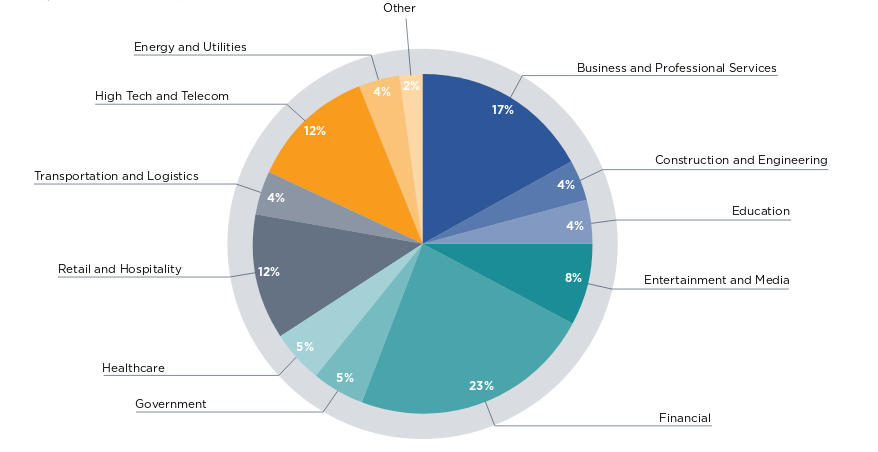
\includegraphics[width=1.0\columnwidth]{graph}
	\caption{Diagram of APT targets}
\end{figure}


%A point of particular concern is the retargeting, in the Americas, 63\% of the companies attacked by an APT, are attacked again last year by the same or similar group. In the Asian and Pacific areas, this is even worse, 78\% of the industries are hacked again. \cite{fireeye_mtrends} \\


%\begin{figure}[ht!]
%	\centering
%	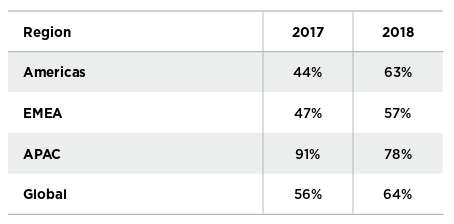
\includegraphics[width=0.5\columnwidth]{retarget}
%	\caption{Retargeting divided by regions}
%\end{figure}

\textit{Advanced persistent threats}, contrary to regular malware, are composed of different phases, each one having an important role. 

The attack is decomposed into smaller steps, for example, if a group of hackers wants to attack a CEO of a given company, they will not send directly to the CEO a phishing email, because he likely has a complex system of security and they would be detected instantly. 
Instead, the first step would hack a person in the same company with lower permissions that can have minor defense mechanisms, or hack some organization that works with the one they want to attack. Once they are established the first computer, they can explore the network infrastructure of the organization, and then decide which action is the next one.
They could cover their track from the log system, locate the data they need, or send a phishing email to the CEO from the owned user.

So how does an APT work? Fireeye described their behavior in six steps \cite{fireeye_anatomy}.

\begin{enumerate}
	\item The adversary gains access into the network infrastructure, installing a malware sent through a phishing email or by exploiting some vulnerability.
	\item Once they comprised the network, the malware scans all the infrastructure looking for other entry points or weaknesses. It can communicate with a Command \& Control server (C\&C) to receive new instructions or to send information.
	\item The malware typically establishes additional points of compromise to ensure that the attack can continue even if a position is closed.
	\item Once the attackers have a reliable connection to the network, they start dumping data such as usernames and passwords, to gain credentials.
	
	\item The malware sends the data to a server where the attackers can receive the information. Now the network is breached.
	
	\item The malware tries to cover its tracks cleaning the log system, but the network is still compromised so the adversary can enter again if they are not detected.
\end{enumerate}

Since APT targets critical infrastructures, governments, organizations, they are mighty and critical. Analysts and researchers work every day to dissect and analyze malware. However, due to their constant increase, researchers can no more handle all of them. 
We proposed a prioritization system to dispatch to analysts only the samples that can be related to an APT campaign. Our system extracts static features from malware samples, to provide a fast and efficient mechanism for APT detection. The main goal of this thesis is to correctly identify samples belonging to the same APT group. Starting from the malware triage \cite{laurenza2017malware} idea presented by Laurenza et al. we tried a different approach using different features from code analysis. Caliskan et al. \cite{caliskan2015anonymizing} inspired us with their technique for de-anonymizing programmers from their executable. We apply the same concept to the malware triage using different tools, and we manage to correctly identify APT classes with promising results. 

We use Ghidra as reverse engineering software to automate the features extraction phase. We rely on Ghidra's scripting capability to automatically extract different information for creating our dataset. Furthermore, we enrich our dataset using the Rich Header information as explained by Dubik\cite{dubyk2019sans}.

We propose different techniques for feature selection and compare their results. In the end, we reduce the number of features by 99.85\% with respect to the original dataset, and we reduce the classification time approximately by 98\%. We obtain great results in both accuracy, precision, recall and f1-score, on average around 95\%. Precision is our main concern since we are developing a prioritization framework, we do not want to dispatch a false postive to human analysts. Some APT classes are detected with a precision of 100\%.


The thesis is organized as follows.
In Chapter \ref{ch:rel-works}, we analyze all the paper that we use to start this thesis. We talk about a novel framework for APT malware prioritization proposed by Laurenza et al. In the next section, we analyze the work made by Caliskan et al. \cite{caliskan2015anonymizing}, where they show how it is still possible to de-anonymize different programmers just relying on executable files. The last work of Dubyk \cite{dubyk2019sans} shows the usage of an undocumented section of the PE header, Rich Header, in malware classification.

Chapter \ref{ch:prelim} introduces the preliminary notions needed for the comprehension of this thesis. It focuses on Reverse Engineering (\textbf{RE}) and shows which documents are useful for an analyst in code analysis. Then we present the state-of-the-art of RE tools, the reasons behind our choice on the tool Ghidra, and all its functionalities useful for code analysis. Furthermore, we present the tools used for machine-learning tasks.

Chapter \ref{ch:feat-cre} focuses on features extraction from the dataset using Ghidra. We shows the different block of features proposed, and for each of them, we present the type of features selected and the extraction process with Ghidra.

Chapter \ref{ch:classif} introduces all the machine-learning models and techniques used. It presents the \textit{RandomForest} and \textit{XGBoost} classifier, and the problem of validating results obtained from a model. Moreover, we present the different techniques for feature selection used to shrink our feature vector.

Chapter \ref{ch:disc} comprehends all the tests we made to evaluate our models. We present in detail the results of feature selection and how we chose the best for our purpose.
Furthermore, we analyze the performances of the two models.

In Chapter \ref{ch:future} we show the future works we could make to improve this thesis. 